
%% bare_conf.tex
%% V1.3
%% 2007/01/11
%% by Michael Shell
%% See:
%% http://www.michaelshell.org/
%% for current contact information.
%%
%% This is a skeleton file demonstrating the use of IEEEtran.cls
%% (requires IEEEtran.cls version 1.7 or later) with an IEEE conference paper.
%%
%% Support sites:
%% http://www.michaelshell.org/tex/ieeetran/
%% http://www.ctan.org/tex-archive/macros/latex/contrib/IEEEtran/
%% and
%% http://www.ieee.org/

%%*************************************************************************
%% Legal Notice:
%% This code is offered as-is without any warranty either expressed or
%% implied; without even the implied warranty of MERCHANTABILITY or
%% FITNESS FOR A PARTICULAR PURPOSE!
%% User assumes all risk.
%% In no event shall IEEE or any contributor to this code be liable for
%% any damages or losses, including, but not limited to, incidental,
%% consequential, or any other damages, resulting from the use or misuse
%% of any information contained here.
%%
%% All comments are the opinions of their respective authors and are not
%% necessarily endorsed by the IEEE.
%%
%% This work is distributed under the LaTeX Project Public License (LPPL)
%% ( http://www.latex-project.org/ ) version 1.3, and may be freely used,
%% distributed and modified. A copy of the LPPL, version 1.3, is included
%% in the base LaTeX documentation of all distributions of LaTeX released
%% 2003/12/01 or later.
%% Retain all contribution notices and credits.
%% ** Modified files should be clearly indicated as such, including  **
%% ** renaming them and changing author support contact information. **
%%
%% File list of work: IEEEtran.cls, IEEEtran_HOWTO.pdf, bare_adv.tex,
%%                    bare_conf.tex, bare_jrnl.tex, bare_jrnl_compsoc.tex
%%*************************************************************************

% *** Authors should verify (and, if needed, correct) their LaTeX system  ***
% *** with the testflow diagnostic prior to trusting their LaTeX platform ***
% *** with production work. IEEE's font choices can trigger bugs that do  ***
% *** not appear when using other class files.                            ***
% The testflow support page is at:
% http://www.michaelshell.org/tex/testflow/



% Note that the a4paper option is mainly intended so that authors in
% countries using A4 can easily print to A4 and see how their papers will
% look in print - the typesetting of the document will not typically be
% affected with changes in paper size (but the bottom and side margins will).
% Use the testflow package mentioned above to verify correct handling of
% both paper sizes by the user's LaTeX system.
%
% Also note that the "draftcls" or "draftclsnofoot", not "draft", option
% should be used if it is desired that the figures are to be displayed in
% draft mode.
%

\documentclass[conference]{IEEEtran}
% Add the compsoc option for Computer Society conferences.
%
% If IEEEtran.cls has not been installed into the LaTeX system files,
% manually specify the path to it like:
% \documentclass[conference]{../sty/IEEEtran}





% Some very useful LaTeX packages include:
% (uncomment the ones you want to load)


% *** MISC UTILITY PACKAGES ***
%
%\usepackage{ifpdf}
% Heiko Oberdiek's ifpdf.sty is very useful if you need conditional
% compilation based on whether the output is pdf or dvi.
% usage:
% \ifpdf
%   % pdf code
% \else
%   % dvi code
% \fi
% The latest version of ifpdf.sty can be obtained from:
% http://www.ctan.org/tex-archive/macros/latex/contrib/oberdiek/
% Also, note that IEEEtran.cls V1.7 and later provides a builtin
% \ifCLASSINFOpdf conditional that works the same way.
% When switching from latex to pdflatex and vice-versa, the compiler may
% have to be run twice to clear warning/error messages.

% *** CITATION PACKAGES ***
%
%\usepackage{cite}
% cite.sty was written by Donald Arseneau
% V1.6 and later of IEEEtran pre-defines the format of the cite.sty package
% \cite{} output to follow that of IEEE. Loading the cite package will
% result in citation numbers being automatically sorted and properly
% "compressed/ranged". e.g., [1], [9], [2], [7], [5], [6] without using
% cite.sty will become [1], [2], [5]--[7], [9] using cite.sty. cite.sty's
% \cite will automatically add leading space, if needed. Use cite.sty's
% noadjust option (cite.sty V3.8 and later) if you want to turn this off.
% cite.sty is already installed on most LaTeX systems. Be sure and use
% version 4.0 (2003-05-27) and later if using hyperref.sty. cite.sty does
% not currently provide for hyperlinked citations.
% The latest version can be obtained at:
% http://www.ctan.org/tex-archive/macros/latex/contrib/cite/
% The documentation is contained in the cite.sty file itself.


%\usepackage{program}
\usepackage{algpseudocode}
\usepackage{graphicx}
\usepackage{hyperref}
\hypersetup{colorlinks=true}


%\usepackage[]{algorithm2e}


% *** GRAPHICS RELATED PACKAGES ***
%
\ifCLASSINFOpdf
  % \usepackage[pdftex]{graphicx}
  % declare the path(s) where your graphic files are
  % \graphicspath{{../pdf/}{../jpeg/}}
  % and their extensions so you won't have to specify these with
  % every instance of \includegraphics
  % \DeclareGraphicsExtensions{.pdf,.jpeg,.png}
\else
  % or other class option (dvipsone, dvipdf, if not using dvips). graphicx
  % will default to the driver specified in the system graphics.cfg if no
  % driver is specified.
  % \usepackage[dvips]{graphicx}
  % declare the path(s) where your graphic files are
  % \graphicspath{{../eps/}}
  % and their extensions so you won't have to specify these with
  % every instance of \includegraphics
  % \DeclareGraphicsExtensions{.eps}
\fi
% graphicx was written by David Carlisle and Sebastian Rahtz. It is
% required if you want graphics, photos, etc. graphicx.sty is already
% installed on most LaTeX systems. The latest version and documentation can
% be obtained at:
% http://www.ctan.org/tex-archive/macros/latex/required/graphics/
% Another good source of documentation is "Using Imported Graphics in
% LaTeX2e" by Keith Reckdahl which can be found as epslatex.ps or
% epslatex.pdf at: http://www.ctan.org/tex-archive/info/
%
% latex, and pdflatex in dvi mode, support graphics in encapsulated
% postscript (.eps) format. pdflatex in pdf mode supports graphics
% in .pdf, .jpeg, .png and .mps (metapost) formats. Users should ensure
% that all non-photo figures use a vector format (.eps, .pdf, .mps) and
% not a bitmapped formats (.jpeg, .png). IEEE frowns on bitmapped formats
% which can result in "jaggedy"/blurry rendering of lines and letters as
% well as large increases in file sizes.
%
% You can find documentation about the pdfTeX application at:
% http://www.tug.org/applications/pdftex


% *** MATH PACKAGES ***
%
\usepackage[cmex10]{amsmath}
% A popular package from the American Mathematical Society that provides
% many useful and powerful commands for dealing with mathematics. If using
% it, be sure to load this package with the cmex10 option to ensure that
% only type 1 fonts will utilized at all point sizes. Without this option,
% it is possible that some math symbols, particularly those within
% footnotes, will be rendered in bitmap form which will result in a
% document that can not be IEEE Xplore compliant!
%
% Also, note that the amsmath package sets \interdisplaylinepenalty to 10000
% thus preventing page breaks from occurring within multiline equations. Use:
%\interdisplaylinepenalty=2500
% after loading amsmath to restore such page breaks as IEEEtran.cls normally
% does. amsmath.sty is already installed on most LaTeX systems. The latest
% version and documentation can be obtained at:
% http://www.ctan.org/tex-archive/macros/latex/required/amslatex/math/


% *** SPECIALIZED LIST PACKAGES ***
%
%\usepackage{algorithmic}
% algorithmic.sty was written by Peter Williams and Rogerio Brito.
% This package provides an algorithmic environment fo describing algorithms.
% You can use the algorithmic environment in-text or within a figure
% environment to provide for a floating algorithm. Do NOT use the algorithm
% floating environment provided by algorithm.sty (by the same authors) or
% algorithm2e.sty (by Christophe Fiorio) as IEEE does not use dedicated
% algorithm float types and packages that provide these will not provide
% correct IEEE style captions. The latest version and documentation of
% algorithmic.sty can be obtained at:
% http://www.ctan.org/tex-archive/macros/latex/contrib/algorithms/
% There is also a support site at:
% http://algorithms.berlios.de/index.html
% Also of interest may be the (relatively newer and more customizable)
% algorithmicx.sty package by Szasz Janos:
% http://www.ctan.org/tex-archive/macros/latex/contrib/algorithmicx/

% *** ALIGNMENT PACKAGES ***
%
%\usepackage{array}
% Frank Mittelbach's and David Carlisle's array.sty patches and improves
% the standard LaTeX2e array and tabular environments to provide better
% appearance and additional user controls. As the default LaTeX2e table
% generation code is lacking to the point of almost being broken with
% respect to the quality of the end results, all users are strongly
% advised to use an enhanced (at the very least that provided by array.sty)
% set of table tools. array.sty is already installed on most systems. The
% latest version and documentation can be obtained at:
% http://www.ctan.org/tex-archive/macros/latex/required/tools/


%\usepackage{mdwmath}
%\usepackage{mdwtab}
% Also highly recommended is Mark Wooding's extremely powerful MDW tools,
% especially mdwmath.sty and mdwtab.sty which are used to format equations
% and tables, respectively. The MDWtools set is already installed on most
% LaTeX systems. The lastest version and documentation is available at:
% http://www.ctan.org/tex-archive/macros/latex/contrib/mdwtools/


% IEEEtran contains the IEEEeqnarray family of commands that can be used to
% generate multiline equations as well as matrices, tables, etc., of high
% quality.


%\usepackage{eqparbox}
% Also of notable interest is Scott Pakin's eqparbox package for creating
% (automatically sized) equal width boxes - aka "natural width parboxes".
% Available at:
% http://www.ctan.org/tex-archive/macros/latex/contrib/eqparbox/

% *** SUBFIGURE PACKAGES ***
%\usepackage[tight,footnotesize]{subfigure}
% subfigure.sty was written by Steven Douglas Cochran. This package makes it
% easy to put subfigures in your figures. e.g., "Figure 1a and 1b". For IEEE
% work, it is a good idea to load it with the tight package option to reduce
% the amount of white space around the subfigures. subfigure.sty is already
% installed on most LaTeX systems. The latest version and documentation can
% be obtained at:
% http://www.ctan.org/tex-archive/obsolete/macros/latex/contrib/subfigure/
% subfigure.sty has been superceeded by subfig.sty.



%\usepackage[caption=false]{caption}
%\usepackage[font=footnotesize]{subfig}
% subfig.sty, also written by Steven Douglas Cochran, is the modern
% replacement for subfigure.sty. However, subfig.sty requires and
% automatically loads Axel Sommerfeldt's caption.sty which will override
% IEEEtran.cls handling of captions and this will result in nonIEEE style
% figure/table captions. To prevent this problem, be sure and preload
% caption.sty with its "caption=false" package option. This is will preserve
% IEEEtran.cls handing of captions. Version 1.3 (2005/06/28) and later
% (recommended due to many improvements over 1.2) of subfig.sty supports
% the caption=false option directly:
%\usepackage[caption=false,font=footnotesize]{subfig}
%
% The latest version and documentation can be obtained at:
% http://www.ctan.org/tex-archive/macros/latex/contrib/subfig/
% The latest version and documentation of caption.sty can be obtained at:
% http://www.ctan.org/tex-archive/macros/latex/contrib/caption/

% *** FLOAT PACKAGES ***
%
%\usepackage{fixltx2e}
% fixltx2e, the successor to the earlier fix2col.sty, was written by
% Frank Mittelbach and David Carlisle. This package corrects a few problems
% in the LaTeX2e kernel, the most notable of which is that in current
% LaTeX2e releases, the ordering of single and double column floats is not
% guaranteed to be preserved. Thus, an unpatched LaTeX2e can allow a
% single column figure to be placed prior to an earlier double column
% figure. The latest version and documentation can be found at:
% http://www.ctan.org/tex-archive/macros/latex/base/

%\usepackage{stfloats}
% stfloats.sty was written by Sigitas Tolusis. This package gives LaTeX2e
% the ability to do double column floats at the bottom of the page as well
% as the top. (e.g., "\begin{figure*}[!b]" is not normally possible in
% LaTeX2e). It also provides a command:
%\fnbelowfloat
% to enable the placement of footnotes below bottom floats (the standard
% LaTeX2e kernel puts them above bottom floats). This is an invasive package
% which rewrites many portions of the LaTeX2e float routines. It may not work
% with other packages that modify the LaTeX2e float routines. The latest
% version and documentation can be obtained at:
% http://www.ctan.org/tex-archive/macros/latex/contrib/sttools/
% Documentation is contained in the stfloats.sty comments as well as in the
% presfull.pdf file. Do not use the stfloats baselinefloat ability as IEEE
% does not allow \baselineskip to stretch. Authors submitting work to the
% IEEE should note that IEEE rarely uses double column equations and
% that authors should try to avoid such use. Do not be tempted to use the
% cuted.sty or midfloat.sty packages (also by Sigitas Tolusis) as IEEE does
% not format its papers in such ways.

% *** PDF, URL AND HYPERLINK PACKAGES ***
%
%\usepackage{url}
% url.sty was written by Donald Arseneau. It provides better support for
% handling and breaking URLs. url.sty is already installed on most LaTeX
% systems. The latest version can be obtained at:
% http://www.ctan.org/tex-archive/macros/latex/contrib/misc/
% Read the url.sty source comments for usage information. Basically,
% \url{my_url_here}.

% *** Do not adjust lengths that control margins, column widths, etc. ***
% *** Do not use packages that alter fonts (such as pslatex).         ***
% There should be no need to do such things with IEEEtran.cls V1.6 and later.
% (Unless specifically asked to do so by the journal or conference you plan
% to submit to, of course. )


% correct bad hyphenation here
% \hyphenation{op-tical net-works semi-conduc-tor}

% paper title
% can use linebreaks \\ within to get better formatting as desired
\title{Leveraging input sparsity to scale random forest}

% author names and affiliations
% use a multiple column layout for up to three different
% affiliations
\author{
\IEEEauthorblockN{Fares Hedayati}
\IEEEauthorblockA{Elance-oDesk\\
                  Dept. of Data Science\\
                  441 Logue Ave, Mountain View, CA 94043\\
                  Email: fares19@elance-odesk.com}
\and
\IEEEauthorblockN{Arnaud Joly}
\IEEEauthorblockA{Dept. of EE \& CS \& GIGA-R\\
                  University of Li�ge\\
                  Belgium\\
                  Email: a.joly@ulg.ac.be
}
\and
\IEEEauthorblockN{Panagiotis Papadimitriou}
\IEEEauthorblockA{Elance-oDesk\\
                  Dept. of Data Science\\
                  441 Logue Ave, Mountain View, CA 94043\\
                  Email: papadimitriou@elance-odesk.com}
}

% conference papers do not typically use \thanks and this command
% is locked out in conference mode. If really needed, such as for
% the acknowledgment of grants, issue a \IEEEoverridecommandlockouts
% after \documentclass

% for over three affiliations, or if they all won't fit within the width
% of the page, use this alternative format:
%
%\author{\IEEEauthorblockN{Michael Shell\IEEEauthorrefmark{1},
%Homer Simpson\IEEEauthorrefmark{2},
%James Kirk\IEEEauthorrefmark{3},
%Montgomery Scott\IEEEauthorrefmark{3} and
%Eldon Tyrell\IEEEauthorrefmark{4}}
%\IEEEauthorblockA{\IEEEauthorrefmark{1}School of Electrical and Computer Engineering\\
%Georgia Institute of Technology,
%Atlanta, Georgia 30332--0250\\ Email: see http://www.michaelshell.org/contact.html}
%\IEEEauthorblockA{\IEEEauthorrefmark{2}Twentieth Century Fox, Springfield, USA\\
%Email: homer@thesimpsons.com}
%\IEEEauthorblockA{\IEEEauthorrefmark{3}Starfleet Academy, San Francisco, California 96678-2391\\
%Telephone: (800) 555--1212, Fax: (888) 555--1212}
%\IEEEauthorblockA{\IEEEauthorrefmark{4}Tyrell Inc., 123 Replicant Street, Los Angeles, California 90210--4321}}

% use for special paper notices
%\IEEEspecialpapernotice{(Invited Paper)}

% make the title area
\begin{document}
\maketitle

\begin{abstract}

Many machine learning tasks involve sparsely representable input space, such as
text data. State-of-the-art tree-based ensemble algorithms and implementation
have focused on tasks with dense input space, while at most emulating random
memory access on sparse input data. We propose a fast and an efficient
splitting algorithm to leverage input sparsity within decision tree methods. We
exploit the a-priori knowledge that each column have very few non-zero
elements and show how learning time is significantly decreased.

\end{abstract}
% IEEEtran.cls defaults to using nonbold math in the Abstract.
% This preserves the distinction between vectors and scalars. However,
% if the conference you are submitting to favors bold math in the abstract,
% then you can use LaTeX's standard command \boldmath at the very start
% of the abstract to achieve this. Many IEEE journals/conferences frown on
% math in the abstract anyway.

% no keywords

% For peer review papers, you can put extra information on the cover
% page as needed:
% \ifCLASSOPTIONpeerreview
% \begin{center} \bfseries EDICS Category: 3-BBND \end{center}
% \fi
%
% For peerreview papers, this IEEEtran command inserts a page break and
% creates the second title. It will be ignored for other modes.
\IEEEpeerreviewmaketitle

\section{Introduction}
% no \IEEEPARstart

Decision trees along with their ensemble variations such as Adaboost, Random
Forest and Gradient Boosting are some of the most robust and widely-used
supervised machine learning and data mining techniques
\cite{breiman1984classification}, \cite{friedman2001greedy,freund1995desicion},
\cite{breiman2001random}. Decision trees can be used both in classification and
regression problems. A tree is a flowchart structure that guides the input
feature vector from the root to a leaf; and the leaf contains the necessary
information for predicting the target variable. The root and each intermediate
inner node correspond to a feature and a splitting criterion that determine the
path of the input down the tree. As learning a tree from training dataset is
known to be NP-complete \cite{hyafil1976constructing}, a heuristic is used
instead. The training dataset is recursively split into homogenous
parts\cite{breiman1984classification}. For the case of classification with
numerical features the training data is recursively partitioned into two parts
by picking a single feature and a threshold that can best split the data into
two homogenous groups in terms of the target variable. The optimality of the
split can be determined by different splitting scores, information gain and
Gini impurity are popular choices. Finding the best threshold of a feature
requires sorting the dataset along the feature and computing the splitting
score for all distinct feature values.

Currently decision trees do not support sparse input in \emph{scikit-learn}
\cite{buitinck2013api,pedregosa2011scikit} and many other packages; the input
is required to be densified first. Memory is not the only challenge, training
time is the real predicament. Training decision trees on datasets with a large
feature dimension such as textual datasets is a challenge as the dataset needs
to be sorted along most of the features at least once. We exploit sparsity of
features to avoid sorting the entire dataset; only nonzero parts of a feature
are sorted and the dataset is rearranged accordingly. Moreover datasets are
stored in a column-wise sparsely-represented matrix for memory efficiency.

\section{Decision Trees}

In this section we briefly go over training decision trees and in the next
section we will show how to tweak this algorithm for support of sparse inputs.
Let $X$ be a matrix of dimension $n \times d$ where $d$ is the dimension of the
feature space and $n$ is the number of training instances, i.e. each row
corresponds to an instance and each column corresponds to a feature. Moreover
we let $Y$ be a vector of size $n$ that contains the target variables, e.g. the
target variable of instance $i$ is at $Y[i]$. Note that the in the function
\emph{FIT} below, $min\_samples\_split$, $min\_samples\_leaf$ and $max\_depth$
are regularization parameters for prevention of overfitting.
$min\_samples\_split$ is the minimum number of training instances required in a
node before a split is carried on the node, $min\_samples\_leaf$ is the minimum
number of instances required in the node and $max\_depth$ is the maximum depth
of the tree. As soon as there are too few instances in the current node or the
best split of the current node leave at least one of the children with too few
instances or the tree becomes too deep no further splitting is carried out and
the current node becomes a leaf node. The tree can be grown alternatively in a
best-first search manner in which case $max\_leaf\_nodes$ is needed as well.
$max\_features$, $splitter$ and $criterion$ are other parameters of the model.
Since our tweak is independent of these parameters we only cover training
decision trees for classification in a depth-first search manner with
information gain. Our change works well with all tree variations. For more
details refer to the latest merge in \emph{scikit-learn} in the tree and
random-forests sections \cite{scikit-learn}.

 To avoid rearranging the whole matrix at the time of sorting, we use an
 auxiliary data structure \emph{samples} to rearrange the indices of the
 training dataset only, keeping $X$ and $Y$ unchanged. Initially
 $samples[i] = i$ for $i \in \{0,1,\cdots, n-1\}$, where $n$ is the number of
 training instances. Each node is specified by two numbers $start$ and $end$.
 These two numbers along with $samples$ specifies the indices of $X, Y$ that
  are in the current node: $samples[start:end]$. Note that we use this name to
  be consistent with \emph{scikit-learn} \cite{scikit-learn}.

\begin{algorithmic}
\Function{FIT}{$start =0, end = n, Node, depth$}
\If {$|end - start| < min\_samples\_split$ or $depth > max\_depth$ }
\State $Node.IsLeaf = True$
\State $Node.Class = \,\,Most\,\, frequent\,\,$
\State $\,\,\,\,\,class \,\,of\,\, Y[samples[start:end]]$
\State \Return $Node$
\EndIf
\State $f, t = BestSplit(start, end)$\\
\State \emph{Rearrange $samples[start:end]$}
\State \emph{such that instances in $samples[start:end]$}
\State \emph{with feature $f$ less than $t$ are before}
\State \emph{those that are great than $t$.}
\State \emph{Let $mid$ be an index in the rearranged samples}
\State \emph{such that $X[samples[start:mid], f]$} are less than
\State \emph{$X[samples[mid:end], f]$}\\

\If {$|mid - start |$ or $|end - mid| <min\_samples\_leaf$}
\State $Node.IsLeaf = True$
\State $Node.Class = \,\,Most\,\, frequent\,\,$
\State $\,\,\,\,\,class \,\,of\,\, Y[samples[start:end]]$
\State \Return $Node$
\EndIf
\State $Node.Feature = f$
\State $Node.Threshold = t$
\State $Node.LeftNode = new \,\, Node()$
\State $Node.RightNode = new \,\, Node()$
\State FIT($start, mid, Node.LeftNode, depth+1$)
\State FIT($mid, end, Node.RightNode, depth+1$)
\State\Return $Node$
\EndFunction
\Function{BestSplit}{start, end}
\State $BestThreshold = 0$
\State $BestScore = -\infty$
\State $BestFeature = 0$
\For{$f \in \{1, \cdots, d\}$}
\State $Sort(X, samples, f, start, end)$
\For{$i \in [start+1:end] $}
\State $t = X[samples[i], f]$
\State $Y_L = Y[samples[start:i]]$
\State $Y_R = Y[samples[i:end]]$.
\State $H_L = \mbox{H}(Y_L)$
\State $H_R = \mbox{H}(Y_R)$
\State $S = H(Y) - \left(\frac{|i - start|}{|end - start|} H_L+\frac{|end - i|}{|end - start|}H_R\right)$
\State Where $H(\,\cdot\,)$ is the entropy
\State $T = t$
\If {$S > bestScore$}
\State $BestScore = S$
\State $BestThreshold = T$
\State $BestFeature = f$
\EndIf
\EndFor
\EndFor \\
\Return $BestFeature, BestThreshold$
\EndFunction
\Function{Sort}{$X, samples, f, start, end$ }
\State \emph{Rearrange $samples[start:end]$}
\State \emph{by sorting $X[samples[start:end], f]$,}
\State \emph{keep $X$ and $Y$ unchanged.}\\
\EndFunction
\end{algorithmic}
\section{Sparsified Decision Trees}


For memory efficiency and taking advantage of sparsity we use a data structure
called \emph{scipy.sparse.csc\_matrix}. This data structure has a common use in
\emph{scikit-learn}. It consists of four parts: \emph{indices}, \emph{indptr},
\emph{data} and $shape$ which contains the dimensions of the matrix. The
indices for column $f$ are stored in:

\begin{equation}
indices[indptr[f]:indptr[f+1]],
\end{equation}
with the corresponding values at
\begin{equation}
data[indptr[f]:indptr[f+1]].
\end{equation}

For example if the $indptr$, $indices$, and $data$ of a $(3 \times 3)$ $csc\_matrix$ be the following:
\begin{align*}
indptr &= [0,2,3,6]\\
indices &= [0,2,2,0,1,2]\\
data &= [1,2,3,4,5,6]
\end{align*}

Then the (dense) matrix itself should be:
$[1, 0, 4$\\
$\,\, 0, 0, 5$\\
$\,\,2, 3, 6]$\\


The only part of the $BestFit$ algorithm of the previous section that changes
is the way we sort the training matrix along a feature. For a given feature $f$
we first find all instances in $samples[start:end]$ where feature $f$ is non-
zero. We, then sort the positive and negative parts separately and rearrange
$samples[start:end]$ accordingly.

The challenge in finding instances in $samples[start:end]$ with non-zero values
of $f$ is that of finding the intersection of $indices[indptr[f]:indptr[f+1]]$
and $samples[start:end]$. Depending on the size of these two sets we can either
perform a binary search or an exhaustive search. For the latter end we need an
additional auxiliary data structure that we call $index\_to\_samples$ which is
a reverse map of $samples$ to its indices, i.e. $index\_to\_samples[j] = i$
when $samples[i] = j$.

If the size of the current node, i.e. $end - start$, is small then we can sort
$samples[start:end]$ and for each instance in $samples[start:end]$ do a binary
search in $indices[indptr[f]:indptr[f+1]]$, this way we can find the
intersection of two sets which is the set of instance of the current node with
non-zero values of feature $f$. On the other hand if the size of the current
node is large, sorting the set might be costly and we do an exhaustive search
instead. Note that we always keep $index\_to\_samples$ up-to-date. For each
instance $index$ in $indices[indptr[f]:indptr[f+1]]$ if
$index\_to\_samples[index]$ is not between $start$ and $end$ then that instance
is not in the current node. So we only keep instances in
$indices[indptr[f]:indptr[f+1]]$ when their corresponding $index\_to\_samples$
is between $start$ and $end$.

We define the following two variables for the current feature $f$
\begin{equation}
n\_indices = indptr[f+1] - indptr[f]
\end{equation}
\begin{equation}
n\_samples = end - start.
\end{equation}

Sorting of $samples[start:end]$ takes $O(n\_samples \times \log(n\_samples))$
and binary search of instances of $samples[start:end]$ in
$indices[indptr[f]:indptr[f+1]]$ takes $O(n\_samples \times \log(n\_indices))$.
Sorting of $samples[start:end]$ happens only once in a $BestSplit$ call for all
candidate features, and the binary search happens for each candidate feature.
On the other hand, the exhaustive search takes $O(n\_indices)$ time. We let $C$
be: $$ n\_samples  \times \log(n\_samples) + n\_samples \times \log(n\_indices)
$$ After testing with different coefficients we came up with the following rule
for the candidate feature $f$:

\begin{algorithmic}
\If{$C  < 0.1 \times n\_indices \,\, $}
\State \emph{ First sort $samples[start:end]$ if it is not already sorted, then for each instance in $samples[start:end]$ carry on a binary search in $indices[indptr[f]:indptr[f+1]]$}
\Else
\State \emph{For each index in $indices[indptr[f]:indptr[f+1]]$ check if its in $samples[start:end]$ by verifying that its $index\_to\_samples$ is between $start$ and $end$.}
\EndIf
\end{algorithmic}

\section{Results}

The first test was carried on the \emph{20 Newsgroups} dataset. The dataset
consists of $20000$ news groups documents distributed across $20$ newsgroups
almost evenly \cite{joachims1996probabilistic}. Training was carried on with
different parameters of $max\_depth$, once with the $csc\_matrix$ sparse matrix
and once with dense matrix. As it can be seen in Figure~\ref{20 news groups},
the training time with dense inputs is much higher than the in their sparse
counterparts. We verified that all $4$ fitted trees are identical.

The second set of tests were carried on synthetic data. Random matrices were
generated with different shapes and densities where a density is the percentage
of non-zero values of a feature. For example a density of $0.1$ means that
every feature is only $10\%$ of the time non-zero. Each matrix was represented
both in a sparse and dense format. Decision trees were fitted once with the
sparse and once in the dense format. Table~\ref{density} contains the training
time of these matrices (the last two columns). As it can be seen in this table
the training time of sparse matrices is much lower that their dense
counterparts when the density of matrix is quite low, i.e. less $0.1$. For no-
quite sparse matrices, e.g. $density = 0.5$, the training time with dense
inputs is lower than their sparse counterparts. As this table suggests
$csc\_matrix$ should only be used in sparse data, e.g. textual data.

\begin{figure}
\centering
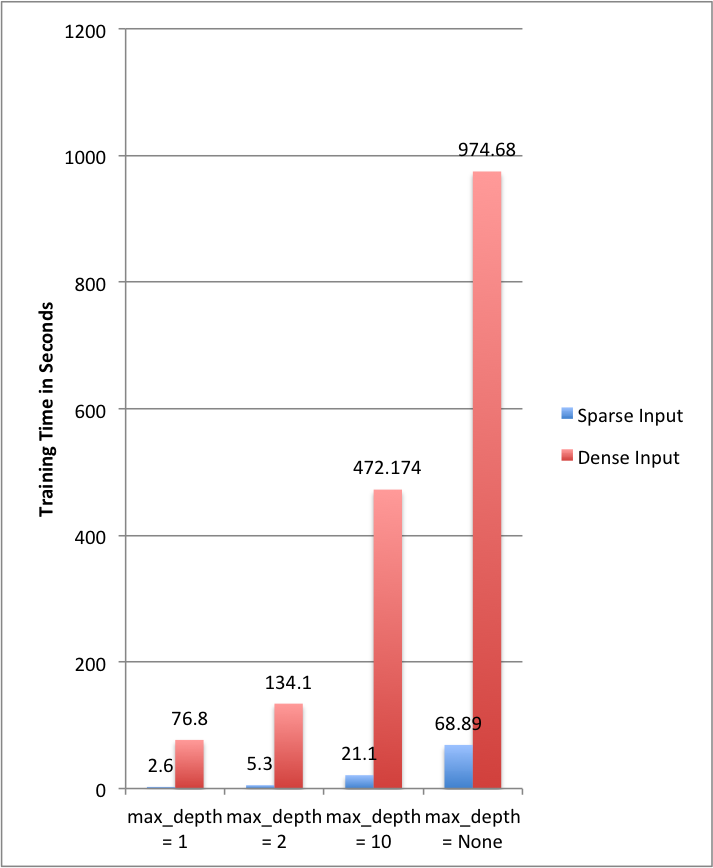
\includegraphics[scale=0.7]{20_news_groups.png}
\caption{Training Time for Different $max\_depth$ on Sparse vs. Dense Input
         (20 News Groups)}
\label{20 news groups}
\end{figure}

\begin{table}[h]
\caption {Training Time in Seconds with Sparse and Dense Inputs} \label{density}
\begin{tabular}{|l|l|l||l|l|l|}
  \hline
Dataset Size	&	Feature Size	&	density	&	 Sparse Input	&	Dense Input	\\
  \hline
10000	  &	1000	&	0.01	&	4.74	&	25.07	\\
100000	&	100	&	0.01	&	7.26	&	24.65	\\
100000	&	1000	&	0.01	&	89.13	&	507.86	\\
10000	  &	1000	&	0.05	&	9.82	&	16.14	\\
100000	&	100	&	0.05	&	21.14	&	28.27	\\
100000	&	1000	&	0.05	&	256.68	&	541.00	\\
10000	  &	1000	&	0.1	&	13.42	&	12.38	\\
100000 	&	100	&	0.1	&	37.81	&	24.65	\\
100000	&	1000	&	0.1	&	437.14	&	370.60	\\
10000	  &	1000	&	0.5	&	28.97	&	14.02	\\
100000	&	100	&	0.5	&	100.22	&	28.13	\\
100000	&	1000	&	0.5	&	949.14	&	383.62 \\
 \hline
\end{tabular}
\end{table}

\section{Conclusion}
The conclusion goes here.

\section*{Acknowledgment} % use section* for acknowledgement

Arnaud Joly is research fellow of the FNRS,
Belgium. This work is supported by PASCAL2 and the IUAP DYSCO, initiated by
the Belgian State, Science Policy Office.

% trigger a \newpage just before the given reference
% number - used to balance the columns on the last page
% adjust value as needed - may need to be readjusted if
% the document is modified later
%\IEEEtriggeratref{8}
% The "triggered" command can be changed if desired:
%\IEEEtriggercmd{\enlargethispage{-5in}}

\bibliographystyle{IEEEtran}
\bibliography{references}

\end{document}


